% ------------------------------------------------------------------------ %
% !TEX encoding = UTF-8 Unicode
% !TEX TS-program = pdflatex
% !TEX root = ../Tesi.tex
% !TEX spellcheck = it-IT
% ------------------------------------------------------------------------ %
%
% ------------------------------------------------------------------------ %
% 	NOME CAPITOLO
% ------------------------------------------------------------------------ %
%
\chapter{Experimental Results}
%
\label{cap:results}

In this chapter are reported the experimental analysis performed to validate the work done for this thesis.\\
First, section \ref{sec:bs-test} contains the experiments conducted over the occupancy monitoring system (BlueSentinel) proposed in chapter \ref{cap:bluesentinel}. The system has been evaluated in terms of accuracy of the localization, responsiveness of the detection and power consumption of the mobile application developed. As we will see, the results confirmed that the proposed approach is suitable to obtain the occupancy monitoring information with a good quality.

Later, section \ref{sec:CAD-test} contains the results obtained from the automatic deployment tool reported in chapter \ref{cap:cad}. The tool has been used to deploy a localization system different from BlueSentinel (a beacons based system) in order to test the general-purpose functionalities and the ability to model different systems. The results include the computational experience of the tool, such as the execution times, and some evaluation metrics of the resulting deployed configuration. These include the cost-effectiveness and the accuracy of the resulting localization system with respect to configuration obtained from different approaches in literature.

\section{Occupancy Monitoring Evaluation}
\label{sec:bs-test}
The occupancy monitoring system presented in chapter \ref{cap:bluesentinel} has been evaluated using data collected from a real-world environment. The system has been set up inside the NECST Lab, located at the basement of DEIB department at Politecnico di Milano.\\
The dimension of the test-bed is 198 squared meters ($9x22m$). The area is subdivided by walls in three separate spaces: a relax room for coffee breaks, a room for meetings and talks, and an open-space with desktop stations.\\
For the installation of the system, before proceed with the training procedure, the administrator needs to identify the regions in which the floor-plan will be partitioned. The dimension of each region will determine the spatial resolution of the occupancy monitoring, as stated in section \ref{sec:occupancy-metrics}. In our setup, we decide to identify a single region for each room in the case of coffee and meeting rooms, while halving the open-space for two main reasons. First, the open-space is large roughly two times the dimension of the other rooms, and this way each region has similar dimensions. Second, because the open-space presents a functional division in two parts between stations occupied by computer security students and by computer architectures students.

The resulting configuration has been used to detect the presence of a user, classifying its position in the best fitting region based on the collected data. The performance and the accuracy of the classification has been evaluated observing manually the ground truth location of the test user.

\begin{figure}[h!tb]
\centering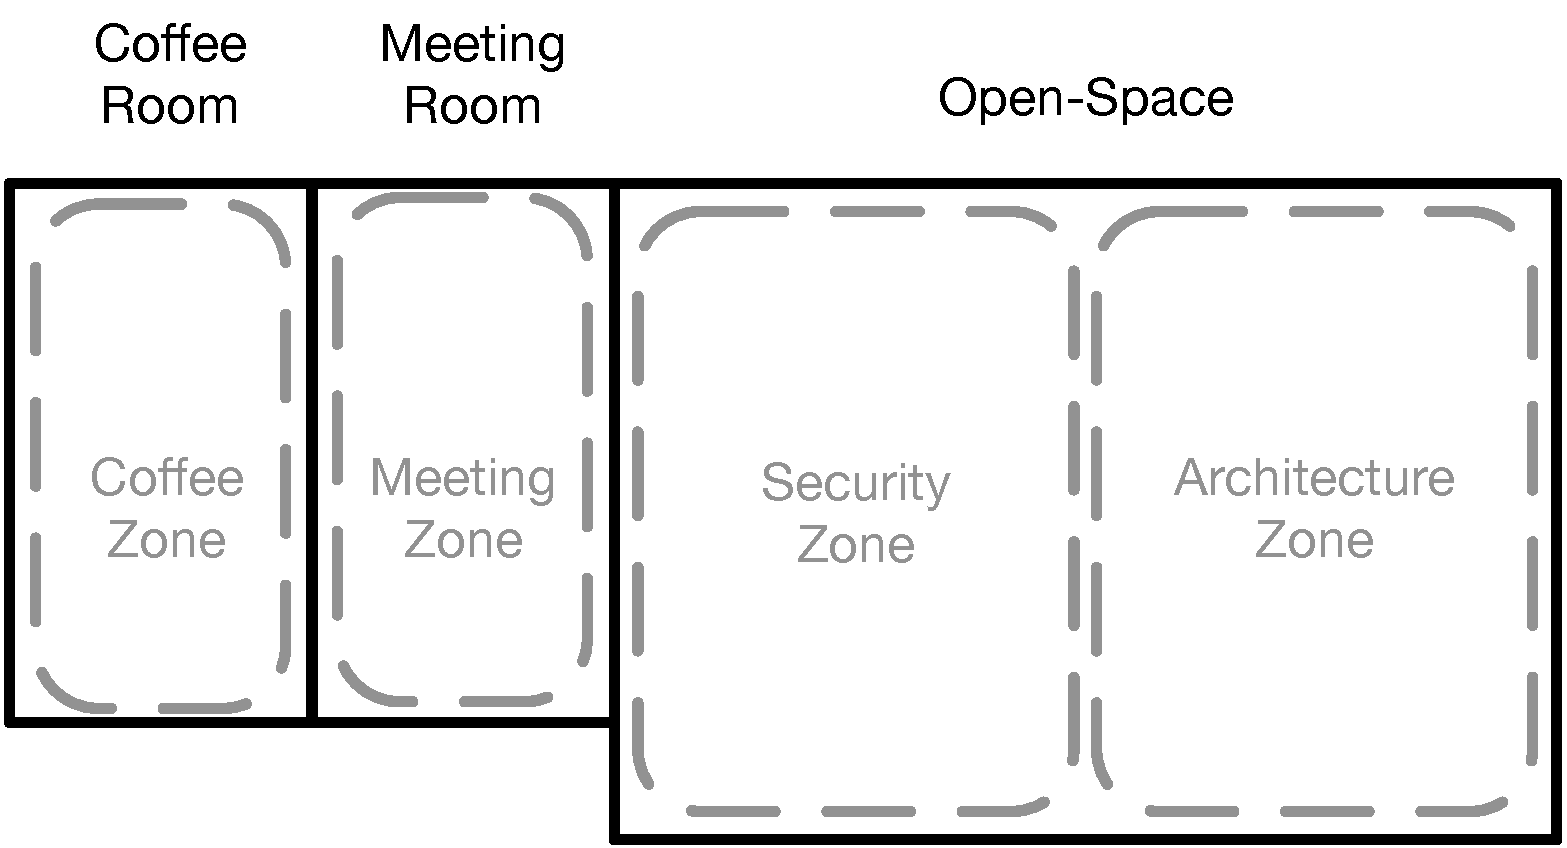
\includegraphics[width=\linewidth]{necst-regions.pdf}
\caption[Floor-plan rooms of the experimental testbed and the regions identified for the occupancy detection.]{Floor-plan rooms of the experimental testbed and the regions identified for the occupancy detection.}
\label{fig:regions}
\end{figure}

\subsubsection{Indoor Environment}
\label{test-env}
The space used for all the test reported in this chapter is that introduced previously and showed in figure \ref{fig:regions}. The perimeter of the laboratory is constituted by reinforced concrete walls, while the walls dividing the three rooms are made in plasterboard.

From the point of view of signal propagation, the environment is characterized by a high level of noise. The space is in most cases high populated, reaching 30 people at the same time ($\approx 1 ~ person / 5m^2$).
Many of these occupants bring in laboratory devices such as smartphones, smartwatches and Bluetooth headphones.
The laboratory equipment includes a high number of wireless devices, such has WiFi access points, Bluetooth beacons, and wireless development boards. Other devices that could interfere with signal transmission and analysis are two microwaves, a projector and a 3D printer.

Summarizing, the wireless communication in our testbed is characterized by lossy and noisy channels, representing a worst case for accuracy measurements.

\subsubsection{Smartphones}
\label{sec:test-phones}
To test the accuracy of the occupancy monitoring system, two Android devices have been employed.
\begin{itemize}
\item The first is a Google Nexus 5 running Android 6.0.1. This device has been used to perform the system training, and to test the localization accuracy when the runtime device is the same of the training.
\item The second is a Samsung I9300 (Galaxy S3) running Android 4.3. This device has been used to test the localization accuracy when the runtime device is different from the device employed for the training.
\end{itemize}
The mobile application running on the devices during test has been explained in detail in section \ref{sec:app}.
The Samsung device has also been used, through a customized battery, to measure precise power consumptions of the mobile application.

%TODO: accennare il fatto che rasp non ha antenna esterna
\subsubsection{WSN prototype}
\label{sec:test-wsn}
Each node of the wireless sensor network has been implemented with Raspberry Pi boards version 3. The operating system running on each board is the Raspbian 4.4 (September 2016) based on Debian 7.0. The software routine running on each sensor node has been detailed in section \ref{sec:wsn}.\\
%posizionamento e quantità dei nodi con immagine (o sketch o cad)
The position and the amount of nodes employed has been obtained using our automatic CAD tool detailed in chapter \ref{cap:cad}. The sketch in figure \ref{fig:wsn-sketch} shows the resulting nodes allocation of four nodes.

\begin{figure}[h!tb]
\centering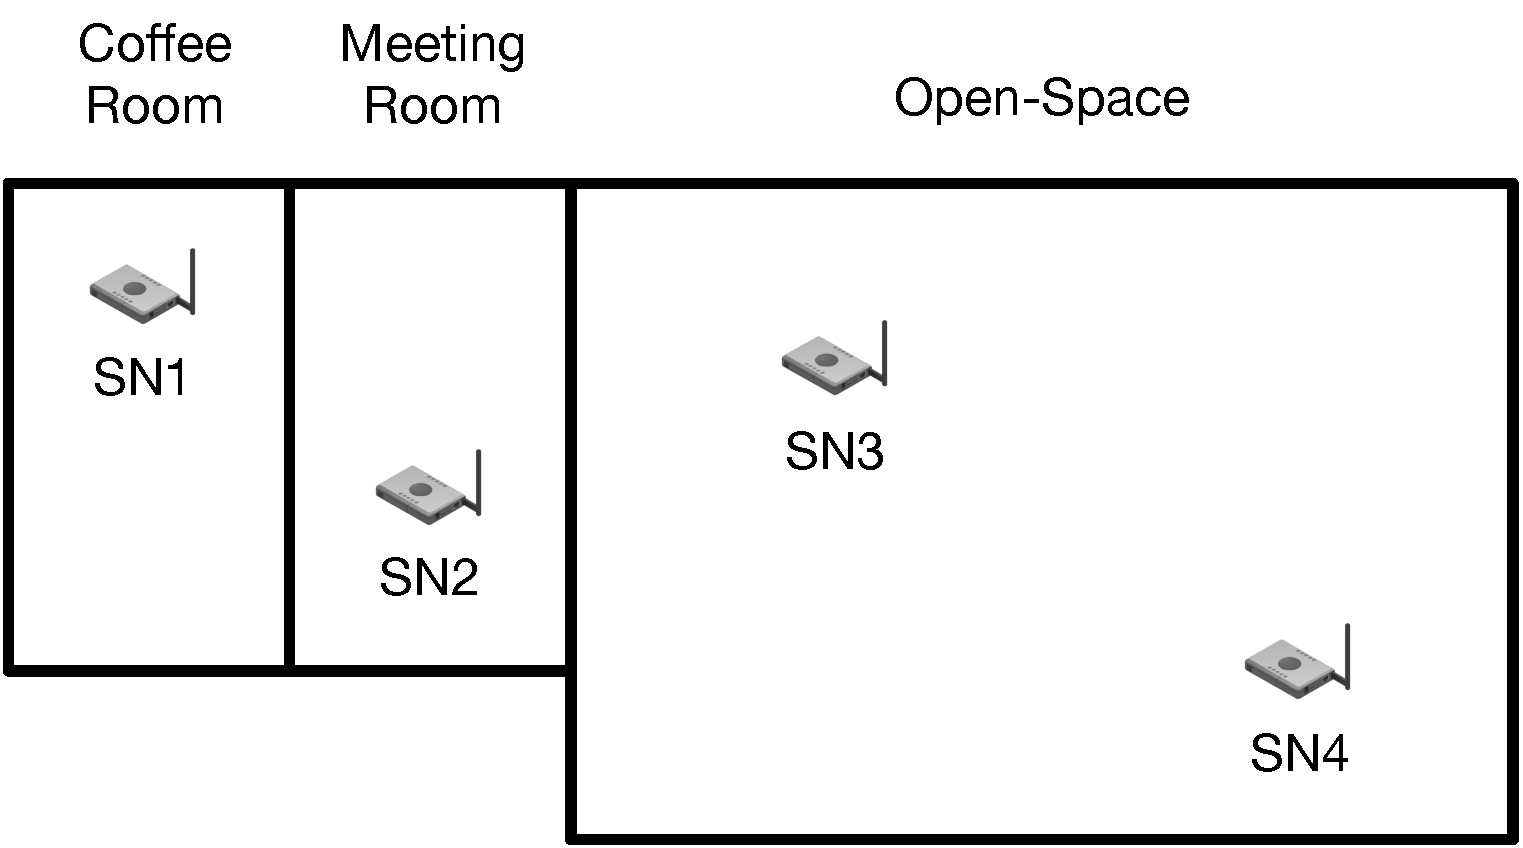
\includegraphics[width=\linewidth]{necst-wsn.pdf}
\caption[Sensor nodes allocation on the floor-plan of the experimental testbed for the occupancy detection.]{Sensor nodes allocation on the floor-plan of the experimental testbed for the occupancy detection.}
\label{fig:wsn-sketch}
\end{figure}

Some of the nodes have been connected to the building LAN using Ethernet sockets, while other were connected using WiFi.
%Power consumption of sensor nodes has been measured using the energy logger 4000 by Voltcraft.
% TODO: togliere o finire

\subsubsection{Back-end}
\label{sub:test-backend}
Since the localization algorithm is performed on the back-end side, the amount of computational resources and the response time of the cloud service determine the responsiveness of the occupancy detection.\\
In our case, the system back-end relies on a cloud platform
\footnote{Parse Cloud service: \url{https://parse.com/}}
that provides free services until a certain load (e.g. the number requests and pushes), while applying different pricing for superior plans.
For this reason, delays of our system at the back-end layer are mainly caused by the plan limits of the cloud service; moving to a custom deployed server with higher computational resources can improve the overall responsiveness.

\subsection{Localization Accuracy}
\label{sec:loc-accuracy}
All the results on the classification algorithms presented in this section have been computed by using the data mining tool Weka \cite{Hall2009}.
During the test we move through the four different regions many times in order to collect a big number of statistical samples.
We have conducted a large number of experiments in order to check if people inside (or outside) a region are correctly recognized by the BlueSentinel system and if the proposed approach can be effectively used to determine the number and the identities of the people inside a particular room.
In the next two sections are reported the results of two classification methods, testing their ability to classify the occupant in the correct region.

\subsubsection{K Nearest Neighbor}
This section reports the results we have obtained by employing the k-Nearest Neighbors algorithm with K equal to 5.
We have computed this values by using a stratified ten-fold cross validation, because of the high number of samples collected.

\begin{table}
\center
\caption[K Nearest Neighbor classification results obtained using the baseline training data.]{K Nearest Neighbor classification results obtained using the baseline training data (section \ref{subsec:algorithms}). Same device refers to measurement obtained using the same device for training and testing. Different device refers to measurement obtained using different devices for training and testing.}
\label{tab:knn-baseline}
\begin{tabular}{ |l|l|l| }
  \hline
  \multicolumn{3}{|c|}{\textbf{KNN Classification - Baseline Dataset}} \\
  \hline
  \textbf{Parameter} & \textbf{Same device} & \textbf{different device}\\
  \hline
  Correctly Classified Instances & 749 (86.09\%) & 635 (72.99\%) \\
  Incorrectly Classified Instances & 121 (13.91\%) & 235 (27.01\%) \\
  Total Number Of Instances & 870 & 870 \\
  Kappa statistic & 0.696 & 0.374 \\
  Mean absolute error & 0.139 & 0.270 \\
  Root mean squared error & 0.373 & 0.519 \\
  True Positive Rate & 86.09\% & 72.99\% \\
  False Positive Rate & 13.91\% & 27.01\% \\
  Precision & 86.09\% & 72.99\% \\
  Recall & 86.09\% & 72.99\% \\
  F-Measure & 86.09\% & 72.99\% \\
  \hline
\end{tabular}
\end{table}

The results in table \ref{tab:knn-baseline} refers to classification performed using baseline RSS data (section \ref{subsec:algorithms}). The results show that KNN is able to classify the occupant in the correct region with an accuracy of 86\% when its device is the same (or has similar transmission power) with the one employed during training. The classifier seems to perform well even if it is pretty simple, leading to a good precision, recall, F-measure and ROC area. The first two metrics evaluate the impact of false positives and false negatives, while the F-measure takes in account both precision and recall. The higher is this metric, the better is the quality of the classifier. Similarly, the receiver operating characteristic (ROC) characterizes the trade-off between hit rate and false-alarm rate in this noisy environment.\\
However, moving to the runtime dataset collected with a different mobile device, the performance suffers a sensible deterioration. In particular, the accuracy is lower than 73\%. This sensible difference is most likely to be caused by the employment of absolute values of RSS, even if different devices transmit signals at different power levels.

\medskip
With the aim to solve this issue, another dataset has been evaluated. In this case, elements of the RSS vectors are not considered as absolute values; instead, a differential value between each couple of RSS is computed and used to build the differential a vector, as explained in section \ref{subsec:algorithms}.
The results that refers to classification performed using differential RSS data are reported in table \ref{tab:knn-diff}.

\begin{table}
\center
\caption[K Nearest Neighbor classification results obtained using the differential training data.]{K Nearest Neighbor classification results obtained using the differential training data (section \ref{subsec:algorithms}). Same device refers to measurement obtained using the same device for training and testing. Different device refers to measurement obtained using different devices for training and testing.}
\label{tab:knn-diff}
\begin{tabular}{ |l|l|l| }
  \hline
  \multicolumn{3}{|c|}{\textbf{KNN Classification - Differential Dataset}} \\
  \hline
  \textbf{Parameter} & \textbf{Same device} & \textbf{different device}\\
  \hline
  Correctly Classified Instances & 757 (87.01\%) & 720 (82.76\%) \\
  Incorrectly Classified Instances & 121 (12.99\%) & 150 (17.24\%) \\
  Total Number Of Instances & 870 & 870 \\
  Kappa statistic & 0.701 & 0.583 \\
  Mean absolute error & 0.118 & 0.159 \\
  Root mean squared error & 0.344 & 0.399 \\
  True Positive Rate & 87.01\% & 82.76\% \\
  False Positive Rate & 13.91\% & 17.24\% \\
  Precision & 87.01\% & 82.76\% \\
  Recall & 87.01\% & 82.76\% \\
  F-Measure & 87.01\% & 82.76\% \\
  \hline
\end{tabular}
\end{table}

The results show that KNN is able to classify the occupant in the correct region with an accuracy of 87\% when its device is the same (or has similar transmission power) with the one employed during training.
The classifier seems to perform well even if it is pretty simple, leading to a good precision, recall, F-measure and ROC area.\\
As expected, moving to the runtime dataset collected with a different mobile device, the performance are lower ($\approx$ 83\%). However, comparing this result to the previous case of baseline data, the classification accuracy has been increased of almost ten percentage points. The differential data approach reveals to be effective to reduce the hardware dependency of samples, and to reduce the correlation between collected data and runtime device.


\subsubsection{Decision Trees}
\label{test-trees}
In this section are presented the results obtained by using decision trees classification, evaluated with a stratified ten-fold cross validation. The specific algorithm employed is detailed in section \ref{subsubsec:trees}. As shown in table \ref{tab:tree-baseline}, for the baseline dataset, the accuracy of the tree algorithm is very similar to the one obtained with the KNN algorithm (table \ref{tab:knn-baseline}). In particular, the accuracy, is slightly lower for same device case (83\%), and almost the same for different device (73.8\%).


\begin{table}
\center
\caption[Decision Trees classification results obtained using the baseline training data.]{Decision Trees classification results obtained using the baseline training data (section \ref{subsec:algorithms}). Same device refers to measurement obtained using the same device for training and testing. Different device refers to measurement obtained using different devices for training and testing.}
\label{tab:tree-baseline}
\begin{tabular}{ |l|l|l| }
  \hline
  \multicolumn{3}{|c|}{\textbf{Decision Trees Classification - Baseline Dataset}} \\
  \hline
  \textbf{Parameter} & \textbf{Same device} & \textbf{different device}\\
  \hline
  Correctly Classified Instances & 726 (83.45\%) & 642 (73.79\%) \\
  Incorrectly Classified Instances & 144 (16.55\%) & 228 (26.21\%) \\
  Total Number Of Instances & 870 & 870 \\
  Kappa statistic & 0.611 & 0.492 \\
  Mean absolute error & 0.136 & 0.241 \\
  Root mean squared error & 0.369 & 0.491 \\
  True Positive Rate & 83.45\% & 73.79\% \\
  False Positive Rate & 16.55\% & 26.21\% \\
  Precision & 83.45\% & 73.79\% \\
  Recall & 83.45\% & 73.79\% \\
  F-Measure & 83.45\% & 73.79\% \\
  \hline
\end{tabular}
\end{table}

Also for tree based classification, the algorithm has been tested with differential data (\ref{tab:tree-diff}).
The results show that decisional trees are able to classify the occupant in the correct region with an accuracy of 85\% when its device is the same (or has similar transmission power) with the one employed during training.
The classifier seems to perform quite well, leading to a good precision, recall, F-measure and ROC area.\\
As expected, moving to the runtime dataset collected with a different mobile device, the performance are lower ($\approx$ 81\%). Unfortunately, with respect to KNN algorithm where the differential data bring a sensible increase in performance for the "different device" case, the previous performance of baseline data has not been increased so much. The differential data approach reveals to be less effective in decisional trees than KNN in order to reduce the hardware dependency of RSS samples.

\begin{table}
\center
\caption[Decision Trees classification results obtained using the differential training data.]{Decision Trees classification results obtained using the differential training data (section \ref{subsec:algorithms}). Same device refers to measurement obtained using the same device for training and testing. Different device refers to measurement obtained using different devices for training and testing.}
\label{tab:tree-diff}
\begin{tabular}{ |l|l|l| }
  \hline
  \multicolumn{3}{|c|}{\textbf{Decision Trees Classification - Differential Dataset}} \\
  \hline
  \textbf{Parameter} & \textbf{Same device} & \textbf{different device}\\
  \hline
  Correctly Classified Instances & 739 (84.94\%) & 706 (81.15\%) \\
  Incorrectly Classified Instances & 131 (15.06\%) & 164 (18.85\%) \\
  Total Number Of Instances & 870 & 870 \\
  Kappa statistic & 0.639 & 0.523 \\
  Mean absolute error & 0.121 & 0.194 \\
  Root mean squared error & 0.349 & 0.440 \\
  True Positive Rate & 84.94\% & 81.15\% \\
  False Positive Rate & 15.06\% & 18.85\% \\
  Precision & 84.94\% & 81.15\% \\
  Recall & 84.94\% & 81.15\% \\
  F-Measure & 84.94\% & 81.15\% \\
  \hline
\end{tabular}
\end{table}


\subsection{Power Consumption}
\label{sec:test-consumption}

As we said in the previous chapters, a key aspect of occupancy monitoring systems based on smart devices is the mobile consumption. In order to make the system non-intrusive on the user habits, the localization needs to preserve the battery energy as more as possible.

A preliminary test on the consumption of Bluetooth Low Energy advertisement have been performed during the feasibility study of the BlueSentinel approach, using an Apple iPhone 6. The test consisted in leaving the smartphone advertising in background (screen off) while observing the discharge, starting from the 100\%. During this test, all the connectivities except the Bluetooth has been disabled to focus exclusively on the advertising consumption. The qualitative test was really impressive, since the phone was able to advertise for 2h:19min without moving from the 100\% of battery level, and for 4h:52min until reach the 90\%.
\smallskip

\begin{figure}[h!tb]
\centering\includegraphics[width=0.7\linewidth]{monsoon.pdf}
\caption{Mobile Device Power Monitor (by Monsoon \textregistered) used to measure the power consumption of the BlueSentinel application.}
\label{fig:monsoon}
\end{figure}

Later, we performed a more precise and quantitative measurement of the power requested at runtime by our developed application.
The test has been performed using the Mobile Device Power Monitor (by Monsoon \textregistered), connected with a Samsung Galaxy S3 through a customized battery (figure \ref{fig:monsoon}). This setup allows to power up the smartphone providing the necessary voltage through the Power Monitor, that bypasses the original battery and measures the power consumption.


\begin{table}[h!tb]
\center
\caption{Power consumption of the mobile device in three different configurations.}
\label{tab:monsoon}
\begin{tabular}{|l|c|c|c|}
  \hline
  \textbf{Configuration} & \textbf{Average current} & \textbf{Voltage} & \textbf{Power chart}\\
  \hline
  All disabled & 2.06 mA & 3.69 V & \ref{fig:monsoon-no} \\
  Only WiFi & 11.78 mA & 3.69 V & \ref{fig:monsoon-wifi} \\
  Only BlueSentinel & 2.57 mA & 3.70 V & \ref{fig:monsoon-bs} \\
  \hline
\end{tabular}
\end{table}

The test conducted with the Power Monitor are summarized in table \ref{tab:monsoon}. All this tests has been performed with the device screen turned off (background mode) since the power requested by the screen is so high that makes the other components negligible. The first configuration tested refers to the smartphone with all the possible wireless connections turned off. Table \ref{tab:monsoon} reports the constant voltage measured and the average current (2.06 mA) of the configuration. Figure \ref{fig:monsoon-no} shows a measured current flow (in violet) very low, where the only affecting component is probably the CPU activity.
The second configuration tested refers to the smartphone with WiFi connection active, while all the other wireless connections turned off. Table \ref{tab:monsoon} reports the constant voltage measured and the average current (11.78 mA) of the configuration. Figure \ref{fig:monsoon-wifi} shows a measured current flow significantly increased from the base case. The last configuration refers to the BlueSentinel advertisement transmission active, with all the other wireless connections turned off. The average current is 2.57 mA, very similar to the baseline configuration. Figure \ref{fig:monsoon-bs} shows the measured current flow where the only affecting component, besides the CPU activity, is the BLE service with a very low profile.

\begin{figure}
\centering
\subfloat[]{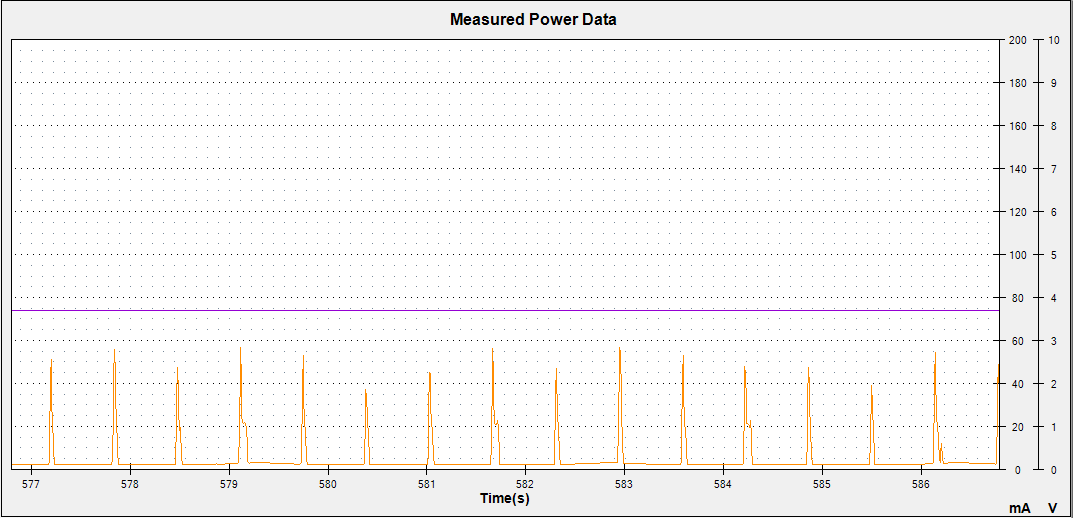
\includegraphics[width=0.85\linewidth]{monsoon-no-conn.png}\label{fig:monsoon-no}}
\newline
\subfloat[]{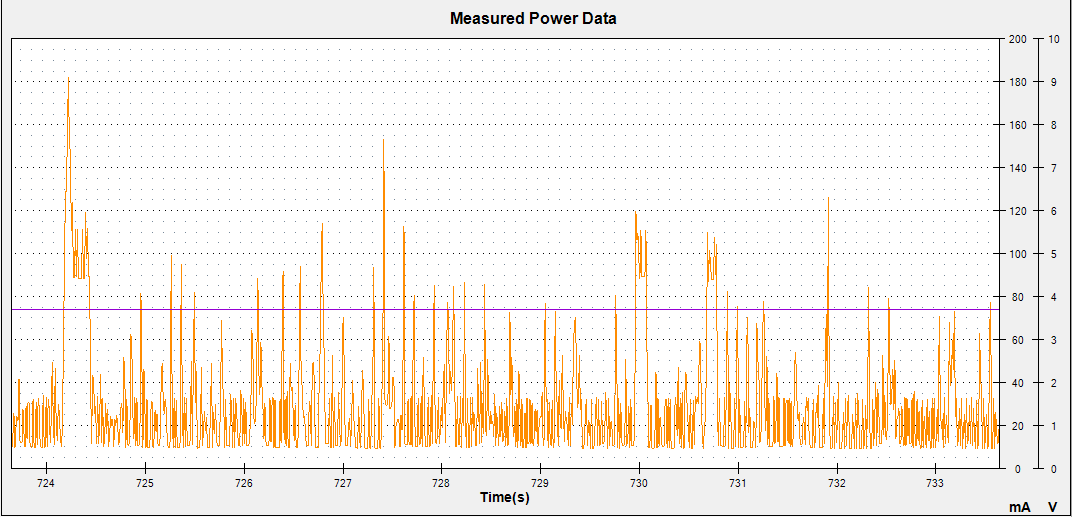
\includegraphics[width=0.85\linewidth]{monsoon-wifi.png}\label{fig:monsoon-wifi}}
\newline
\subfloat[]{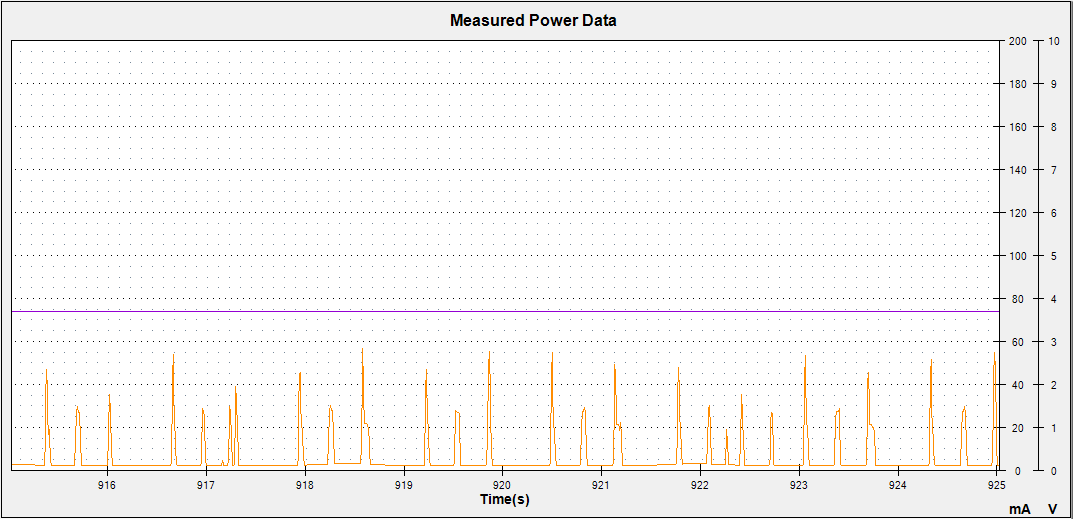
\includegraphics[width=0.85\linewidth]{monsoon-bs.png}\label{fig:monsoon-bs}}
\caption[Power consumption of a Samsung Galaxy S3.]{Power consumption of a Samsung Galaxy S3: orange line represents current, violet line represents voltage. \protect\subref{fig:monsoon-no} All connections disabled. \protect\subref{fig:monsoon-wifi} Only WiFI enabled. \protect\subref{fig:monsoon-bs} Only the BlueSentinel advertisement enabled.}
\label{fig:monsoon-graph}
\end{figure}


\subsection{Responsiveness Test}
\label{test-resp}
An important evaluation metric of the occupancy detection system is the time spent between the transition of a user in a new region and the instant in which the transition is detected. This metric represents the ability of the system to provide a real-time service.

Before discussing the results is important to notice how many factors affect the responsiveness. First, the BLE advertisement frequency of the mobile device. Then, on each sensor node, the signal is filtered to reduce fluctuations (section \ref{sec:wsn}) introducing a considerable delay. Later, data needs to be sent over HTTP requests. Finally, the back-end computation could introduce delays for three different causes: a possible slowdown of the cloud service, the execution time of the classification algorithm, and a possible false negative detection of the algorithm when the occupant is still very close to the previous region.

\newcolumntype{Y}{>{\centering\arraybackslash}X}
\begin{table}[h!tb]
\center
\caption{Responsiveness of the system using different time windows for the EWMA signal filter.}
\label{tab:resp}
\begin{tabularx}{0.85\linewidth}{|Y|Y|Y|}
  \hline
  \textbf{EWMA Time Window [sec]} & \textbf{Average System Delay [sec]} & \textbf{Delay Standard Deviation [sec]} \\
  \hline
  0.5 & 5.202 & 1.21 \\
  1.0 & 3.915 & 0.99 \\
  1.5 & 3.761 & 1.08 \\
  2.0 & 4.420 & 0.95 \\
  \hline
\end{tabularx}
\end{table}

Table \ref{tab:resp} reports the average system delay experienced using different time windows for the signal filtering. The tabulated values suggest that a time window of 0.5 seconds is too short to smooth the signal fluctuations, causing false negative detections that increase the overall delay. A time window of 2.0 seconds is large and the RSS samples are pushed to the back-end in a discontinuous way. The time window of 1.5 seconds performs better. The resulting average delay of 3.761 seconds is not impressive; however as introduced before, it can be reduced by improving the system implementation at different levels, from mobile to server layer.

The values reported in table \ref{tab:resp} have been computed using the tree based classification.
%As stated in section \ref{sec:loc-accuracy}, the tree-based classification algorithm performs better during the run-time phase, thus it has to be preferred every time the cost of the offline training phase does not affect the tree overall quality of the system (which usually happens in most cases, where the physical layout of the building changes quit rarely).
From the point of view of timing performance, the time required to the tree-based classification algorithm to produce the results is in the order of few milliseconds, while the ones of the KNN algorithm are in the order of tens of milliseconds. Thus, even though both the approaches meet the quasi real-time performance typically required by this kind of applications, the tree-based algorithm represents the fastest solution, being around one order of magnitude better than KNN.


\section{Automatic Nodes Deployment Results}
\label{sec:CAD-test}

In this section are reported the experimental results of the CAD tool proposed in chapter \ref{cap:cad}.
Presented results are initially focused on the usability of the tool, testing the ability to provide a solution in a reasonable time. Then, the performances of the model have been evaluated, in terms of localization accuracy through realistic indoor environment experiments, and in terms of cost-effectiveness of the suggested deployments.

\subsection{Computational Experience}\label{subsec:comp_res}
The tool has been been evaluated running several different configurations. Every test reported in this section has been executed with a spatial resolution of the floor plan equal to 1 meter.  A first analysis can be done on the execution times of the proposed solution. Although the execution time can be tuned by the parameter $R_{max}$, which represent the maximum number of restarts of the VNS algorithm, an idea on the order of magnitude is given by Figure~\ref{fig:time}, where the time is represented as a function of the floor-plan dimension.
\begin{figure}[h!tb]
\centering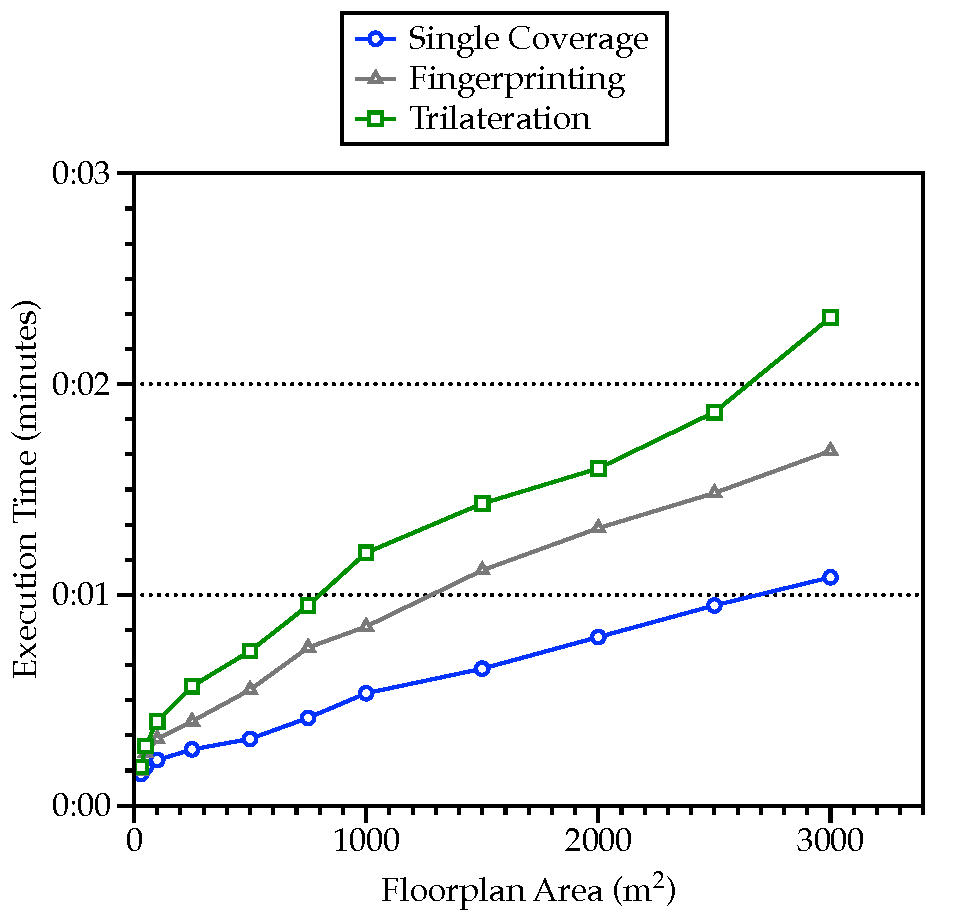
\includegraphics[scale=0.55]{exec_times.pdf}
\caption{Execution time of the tool with floor plans of different areas, for each covering technique ($R_{max} = 20$, $target = 95\%$, $r_t=8$).}
\label{fig:time}
\end{figure}
In the given example, $R_{max}$ has been fixed to 20 restarts, the $target$ coverage equals to 95\% of the total area, a single node type available with a range of 8 meters, covering floor-plans with rectangular areas. The graph shows that for single coverage, the execution time is low even for areas of 3000 squared meters. For trilateration and fingerprinting, the execution times become high from floor-plan of $2500~m^2$. However, the tests represent a bad case in which the map dimension is very large while the node range available and the spatial resolution are small (respectively 8m and 1m). Increasing the range or the resolution, the instance of the problem decrease, resulting in faster executions.

A key aspect that characterizes the goodness of the proposed approach is the improvement of the objective function achieved by the VNS algorithm with respect to the first Greedy configuration. For this test we have run the tool several times with a floor-plan area of $2500~m^2$ and a node range of $12m$. The number of reference nodes allocated is determined by the Greedy procedure and increase with $S$, while the number of VNS restarts $R_{max}$ has been fixed to 35.

\begin{figure}[h!tb]
\centering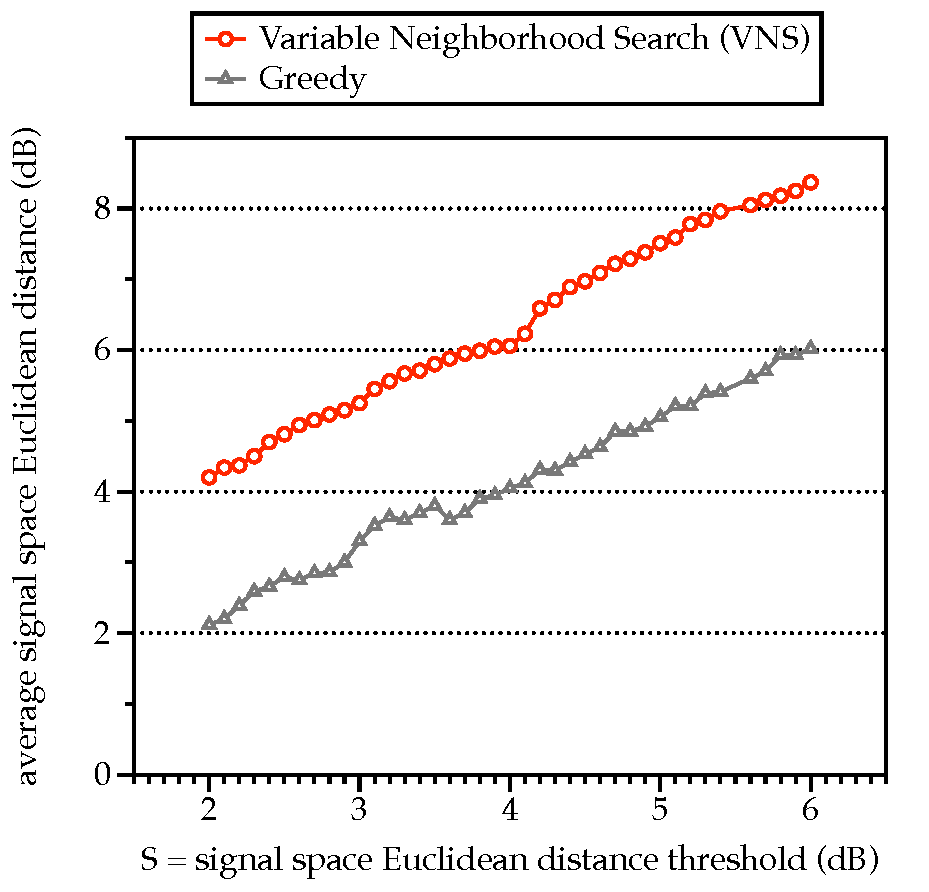
\includegraphics[scale=0.55]{greedy_vs_vns.pdf}
\caption{Average signal space Euclidean distance ($z$) obtained with the Greedy execution and compared with the $z$ value after the VNS optimization. $z$ values expressed as a function of the threshold $S$. Floor-plan area $=2500~m^2$, $R_{max} = 20$, $target = 100\%$, $r_t=12$}
\label{fig:greedy_vns}
\end{figure}

In Fig.~\ref{fig:greedy_vns} are reported the value of $z$, i.e. the average signal space Euclidean distance obtained with the first Greedy execution, compared with the $z$ value after the VNS optimization. The graph reports the $z$ values as a function of the threshold $S$, described in section~\ref{subsec:greedy} as the minimum value of average signal space Euclidean distance ($z$) required during the Greedy procedure. The graph shows that moving the threshold within the range $(2,6)$dB the VNS is able to improve the $z$ value constantly around 2 dB.
Although the VNS improvement is not astonishing for what regard the average value, Fig.~\ref{fig:greedy_vns2} shows that the variance is strongly improved. This has been achieved moving from the objective function $z$ used in Greedy procedure to the $Z$ function of the VNS. The $Z$ objective function has in fact the purpose to provide as many target location as possible with a high signal space Euclidean distance w.r.t. the surrounding locations.

\begin{figure}[h!tb]
\centering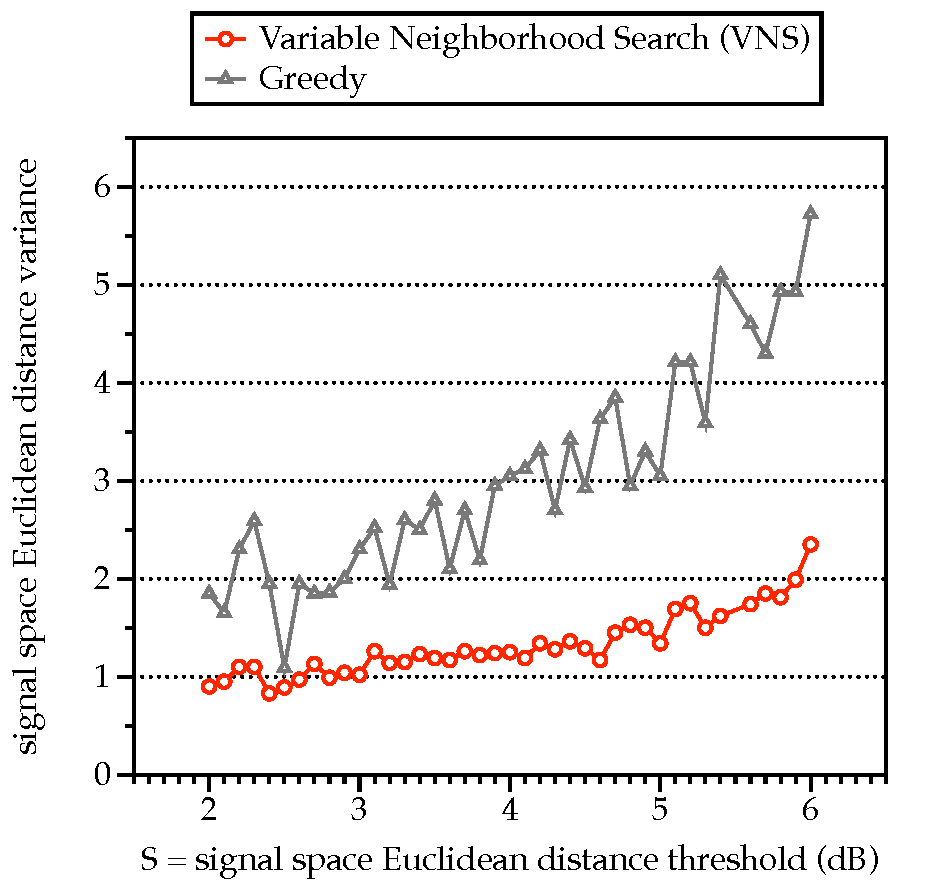
\includegraphics[scale=0.55]{greedy_vs_vns2.pdf}
\caption{Signal space Euclidean distance variance obtained with the Greedy execution and compared with the $z$ value after the VNS optimization. Values expressed as a function of the threshold $S$. Floor-plan area $=2500~m^2$, $R_{max} = 20$, $target = 100\%$, $r_t=12$}
\label{fig:greedy_vns2}
\end{figure}

\begin{figure}
\centering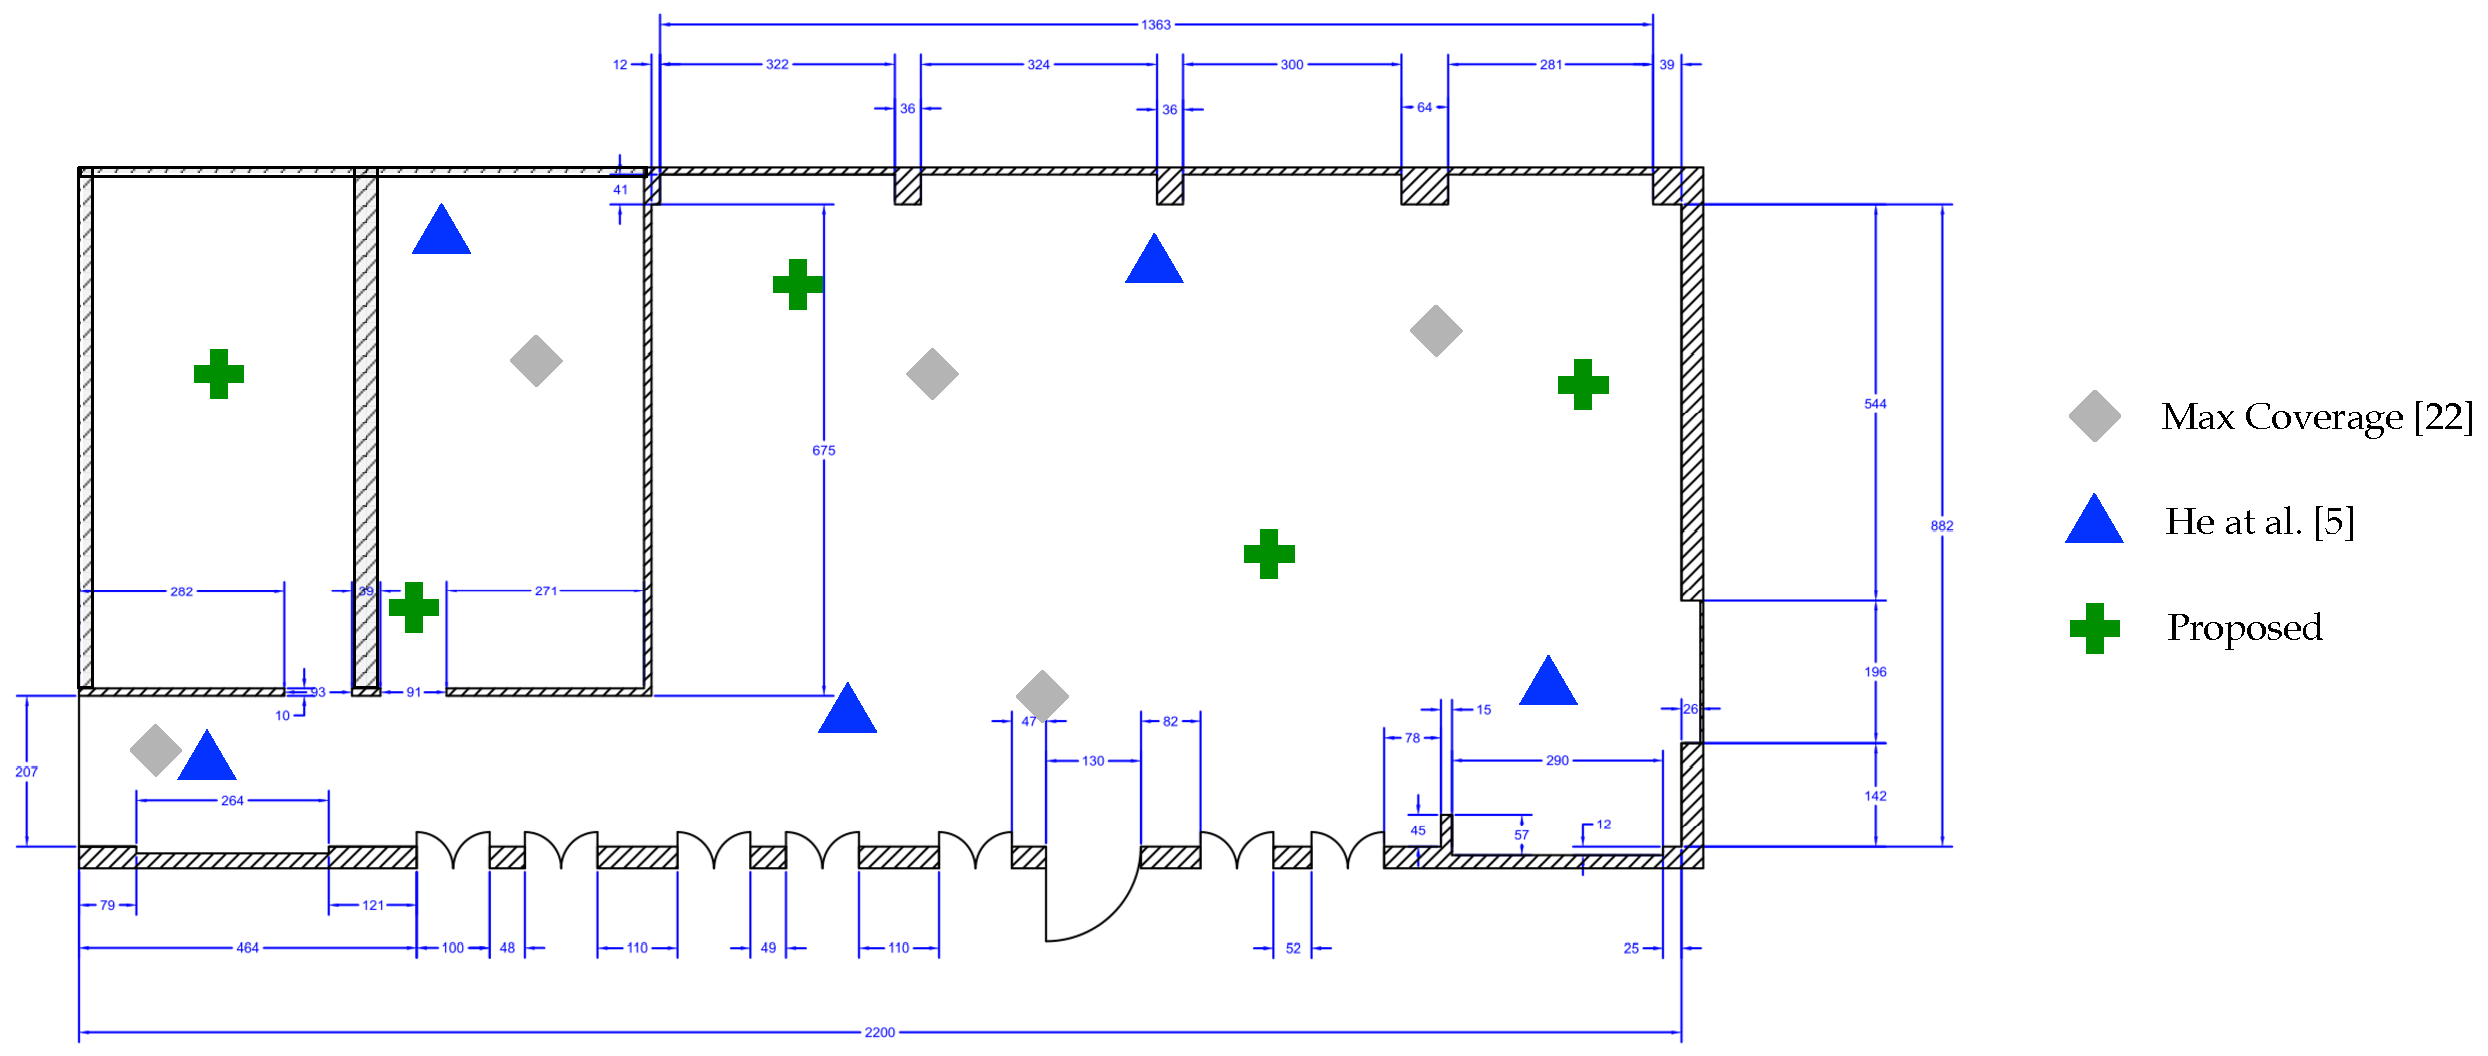
\includegraphics[width=\linewidth]{necst.pdf}
\caption[NECST Lab floor-plan used as indoor environment testbed for deployments evaluation.]{NECST Lab floor-plan, located at the basement of DEIB department at Politecnico di Milano. Each allocation corresponds to a BLE beacon with a range of 7 meters. Green crosses indicates allocations provided by our algorithm, gray rhombus represent allocations from \cite{He2011} while blue triangle positions have been computed maximizing the coverage \cite{Kouakou2010a}.}
\label{fig:necst}
\end{figure}

\subsection{Experimental Setup and Accuracy Evaluation}
The proposed tool was evaluated using data collected from a real-world environment, the NECST Lab, located at the basement of DEIB department at Politecnico di Milano. The dimension of the test-bed is 198 squared meters ($9x22m$). We collected Bluetooth Low Energy (BLE) signal data coming from BLE beacons with a coverage radius of 7 meters. Signal data has been collected using a Nexus 5 smartphone running Android 6.0.1.
First, the NECST Lab floor-plan has been designed using our tool, obtaining the optimal number of beacons ($|N|=5$) and their allocation for fingerprinting localization. $R_{max}$ has been fixed to 20 restarts, the $target$ coverage equals to 100\% of the total area, a single node type available with a range of 7 meters, and the threshold $S=4,5$.
We collected 40 training samples for the localization algorithm using the obtained allocation. Then, the test samples were collected at distinct positions changing the phone orientation and the way in which user was keeping it, for example by hand or in a pocket. For the entire duration of training and test phase, the number of occupants and their enabled wireless devices has changed, from a minimum of 3 to a maximum of 17 people. This variation affects the accuracy performances, but at the same time contributes in obtaining realistic results. The training and test phase has been repeated with two configurations coming from different allocation algorithms: maximization of the coverage \cite{Kouakou2010a} and the allocation algorithm proposed by He at al. in \cite{He2011}. For these two algorithms, the number of employed nodes has been fixed to 5.
KNN with $K=3$ has been employed as the fingerprinting algorithm.

\begin{figure}[h!tb]
\centering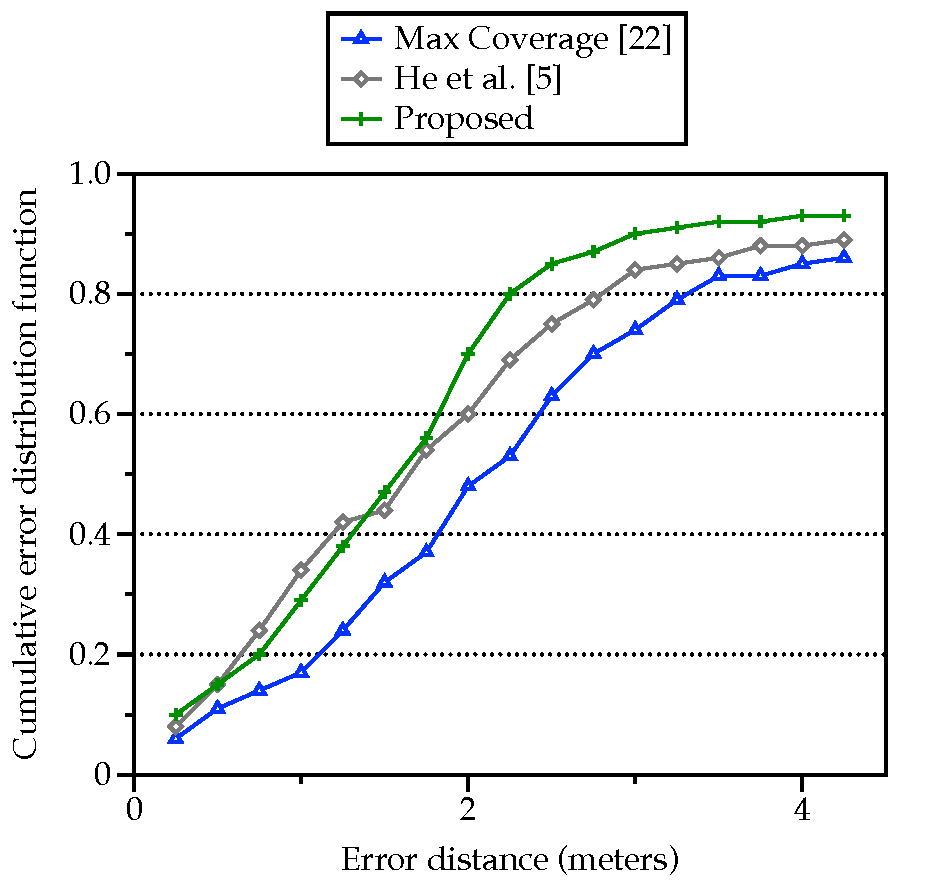
\includegraphics[scale=0.55]{loc_error.pdf}
\caption{Cumulative error distribution function experienced by our approach ad compared with two different solutions from the state-of-the-art.}
\label{fig:loc_error}
\end{figure}

A first result is showed in figure \ref{fig:loc_error}. The cumulative error distribution function shows that from 1.5 meters our approach performs better. Under 1.5 meters, He at al. approach performs better, but the difference in accuracy is marginal.

\begin{figure}[h!tb]
\centering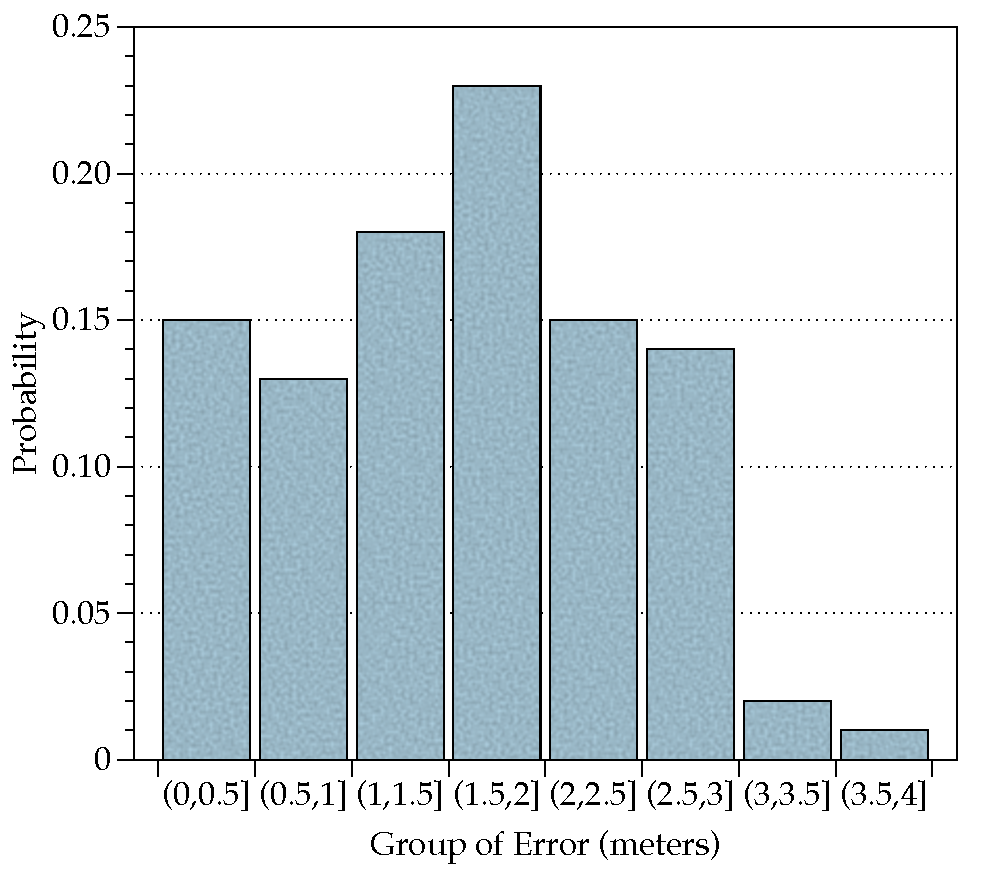
\includegraphics[scale=0.52]{group_errors.pdf}
\caption{Mean positioning accuracy of the proposed allocation algorithm divided into different error ranges.}
\label{fig:group_errors}
\end{figure}

Figure~\ref{fig:group_errors} shows the mean positioning accuracy divided into different error ranges: $( 0,0.5],$ $(0.5,1],$ $(1,1.5],$ $(1.5,2],$ $(2,2.5],$ $(2.5,3],$ $(3,3.5],$ $(3.5,4]$. It's possible to notice that the majority of the localization errors appears within the $(1.5,2]$ meters.
The test-bed floor-plan, composed by 3 rooms, has been reported in figure \ref{fig:necst}. Green crosses indicates allocations provided by our algorithm, gray rhombus represent allocations from \cite{He2011} while blue triangle positions have been computed maximizing the coverage \cite{Kouakou2010a}.

\subsection{Cost-effectiveness Analysis}
A feature of our tool interesting for testing is the possibility to obtain solutions from mixed node types, with different characteristics and costs. In particular, given two types $t_1$ and $t_2$ characterized by two ranges $r_i$, and two costs $c_i$, it's possible to compare the total cost of a homogeneous solution with the cost of a mixed solution. Given a baseline type of node with a range $r_1=8~m$ and a cost of $c_1=60~\$$, we can assume the presence on the market of a second type of hardware, with the half of the range distance ($r_2=4~m$). The area covered by $t_1$ ($\approx200~m^2$) is four times bigger than the coverage of $t_2$ ($\approx50~m^2$). In order to obtain a fair test, the cost of $t_2$ should be \(c_2 \geq c_1/4\), and so we set $c_2=20~\$$. This test has been performed with a $target$ coverage of 95\% on a rectangular map of $1000~m^2$.

From Table \ref{tab:costs} it's possible to observe that, although hardware nodes of type $t_2$ have a lower convenience in terms of $\frac{area}{price}$ ($t_1$ outperform $t_2$ in homogeneous solutions), the mixed strategy can use the smaller range nodes to reduce the total cost. 
\begin{table}[h!tb]
  \centering
  \renewcommand{\arraystretch}{1.5}
  \caption{Cost of homogeneous and mixed solutions ($A=1000~m^2$, $target=95\%$, $r_1=8m$, $r_2=4m$, $c_1=60\$$, $c_2=20\$$).}
  \label{tab:costs}
  \begin{tabular}{|c|c|c|c|}
    \hline
    \multirow{2}{*}{\textbf{Node types}} & \multicolumn{3}{c|}{\textbf{Solution Costs (in \$)}}\\
    \cline{2-4}
    & Single & Trilateration & Fingerprinting\\
    \hline
    $T=\{t_1\}$ & 480 & 1440 & 840\\
    $T=\{t_2\}$ & 500 & 1620 & 880\\
    $T=\{t_1, t_2\}$ & 440 & 1280 & 760\\ \hline
  \end{tabular}
\end{table}
This because less powerful nodes of type $t_2$ are employed to cover small portions of the floor-plan, like corners or small regions left uncovered by the larger range nodes.

The amount of saving in the total cost of the mixed solution doesn't depend only on the nodes range and price, but also on the irregularity of the floor plan perimeter. A distinguish feature of the proposed tool respect to other works is the possibility to cover spaces that are not necessarily rectangular or squared. The level of irregularity of a floor plan can be identified by the minimum number of rectangles that compose the shape. In Figure \ref{fig:irregularity} for example, the index of the floor plan irregularity is $I=4$. 
\begin{figure}[h!tb]
\centering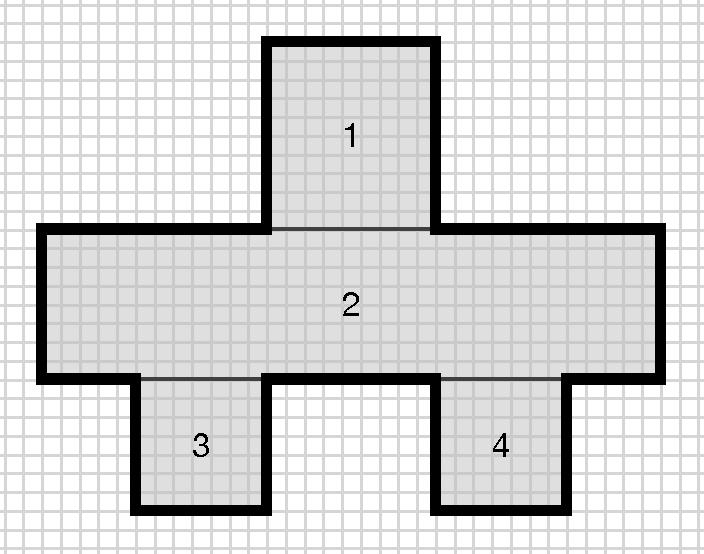
\includegraphics[scale=0.47]{irregularity.pdf}
\caption{Irregularity of the floorplan perimeter summarized by the minimum number of rectangles.}
\label{fig:irregularity}
\end{figure}
We experimented the behavior of the tool increasing the level of irregularity, while maintaining a constant total area of $1000~m^2$. The test has been done with the same nodes configuration used in table~\ref{tab:costs} (homogeneous $T=t_1$, mixed $T=t_1,t_2$). The results shown in Table~\ref{tab:irregularity} proven that increasing the floor-plan irregularity, the cost difference between homogeneous and mixed solution becomes higher. This is caused by the increasing number of corners in the map, that can be covered with less powerful nodes.
%\newcolumntype{Y}{>{\centering\arraybackslash}X}
\begin{table}[H]
  \centering
  \renewcommand{\arraystretch}{1.2}
  \caption{Cost differences (in \$) between homogeneous and mixed solution increasing the floor plan irregularity (area fixed to $1000~m^2$).}
  \label{tab:irregularity}
  \begin{tabularx}{\columnwidth}{|c|YY|YY|YY|}
    \hline
    \multirow{2}{0.55cm}{\textbf{$~~I$}} & \multicolumn{2}{c|}{\textbf{Single}} & \multicolumn{2}{c|}{\textbf{Trilateration}} & \multicolumn{2}{c|}{\textbf{Fingerprinting}}\\
    \cline{2-7}
    & homogen. & mixed & homogen. & mixed & homogen. & mixed\\
    \hline
    1 & 480 & 440 & 1440 & 1280 & 840 & 760\\
    2 & 480 & 440 & 1500 & 1320 & 840 & 780\\
    4 & 600 & 500 & 1560 & 1380 & 900 & 820\\
    8 & 720 & 580 & 1680 & 1480 & 1200 & 920\\
    \hline
  \end{tabularx}
  \end{table}
In conclusion, experimental results show that for most of the problem instances, a solution can be obtained in reasonable execution times. Depending on the available hardware types, homogeneous solutions could be improved with the employment of different type of nodes.

%
% -----------------------------END------------------------------------- %